\documentclass[12pt]{article}
\setlength{\textwidth}{17cm}
\setlength{\textheight}{24cm}
\setlength{\topmargin}{-2cm}
\setlength{\footskip}{1cm}
\setlength{\evensidemargin}{0cm}
\setlength{\oddsidemargin}{0cm}
\setlength{\parindent}{1cm}

\usepackage{allrunes}
\usepackage{amsmath}
\usepackage[magyar]{babel}
\usepackage[T1]{fontenc}
\usepackage[utf8]{inputenc}
\usepackage{fixltx2e}
\usepackage{multirow}

\usepackage[hyphens]{url}
\usepackage[unicode,colorlinks=true,breaklinks]{hyperref}
%\usepackage[dvips]{hyperref}
%should display links, but it does not work with \H accent
%and formulas in section titles

\hypersetup{colorlinks,linkcolor=blue,urlcolor=magenta,citecolor=magenta}
%Breaks long url`s in text, while keeping it one link:

\usepackage{amsfonts}
\usepackage{amsthm}
\usepackage{amssymb}


\theoremstyle{plain}
\usepackage{graphicx}

%\usepackage{gensymb}
\usepackage{float}

% For bra-ket notation
\usepackage{braket}

%% New commands
\newcommand{\dd}{\textrm{d}}

%% Pauli matrices
\newcommand{\sigx}{\sigma_x}
\newcommand{\sigy}{\sigma_y}
\newcommand{\sigz}{\sigma_z}

\newcommand{\paulix}{
    \left( \begin{array}{cc}
        0 & 1 \\
        1 & 0
    \end{array}
    \right)
}

\newcommand{\pauliy}{
    \left( \begin{array}{cc}
        0 & -i \\
        i & 0
    \end{array}
    \right)
}

\newcommand{\pauliz}{
    \left( \begin{array}{cc}
        1 & 0 \\
        0 & -1
    \end{array}
    \right)
}


\begin{document}
\title{7. tétel}
\author{Horváth Benedek}

\maketitle


\newpage
\begin{abstract}
    Molekuláris dinamika, Verlet- és sebesség-Verlet-algoritmus, termodinamikai mennyiségek meghatározása és relaxáció.
\end{abstract}


\section{Bevezetés}

A molekuladinamika hatékony és széles körben alkalmazott szimulációs eljárás kristályos, amorf, folyékony és gáz halmazállapotú anyagok, sőt, makromolekulák fizikai és kémiai tulajdonságainak meghatározására, illetve időfüggő mikroszkopikus folyamatok, mint például diffúzió modellezésére. A módszer hatékonysága abban rejlik, hogy az atomok belső -- kvantummechanikával leírható -- szerkezetét elhanyagolva azokat klasszikus és pontszerű objektumoknak tekintjük, és egyenként követjük a trajektóriájukat a klasszikus newtoni mozgásegyenletük numerikus integrálásával. A módszer tehát teljesen determinisztikus -- ellentétben a sokrészecske-szimulációk egy másik típusával, a Monte Carlóval. Az atomok között párkölcsönhatásokat veszünk figyelembe, amit valamilyen potenciállal írunk le. Az egyszerű Lennard-Jones potenciáltól kezdve az igen bonyolult, molekulák rotációs és vibrációs módusait, illetve belső polarizációját is modellező erőtereken át a kovalens kötések létrejöttét és felbomlását is figyelembe vevő reaktív erőterekig igen sokféle potenciált használnak a szimulációkban. Közös tulajdonságuk, hogy elméleti -- gyakran kvantummechanikai, pl. sűrűségfunkcionál-elmélet, Hartree-Fock módszer -- háttérszámolásokkal vannak validálva, többparaméteres függvényillesztés révén. (Részletekre itt most nem térek ki, az érdeklődők számára szemléltető példaként ajánlom a szén, hidrogén és oxigén atomokat tartalmazó rendszerek összetett Reactive Force Field típusú potenciáljáról szóló publikációt \cite{KimberlyChenoweth2008}.) A párkölcsönhatások számolása és a részecskék egyenkénti mozgatása komolyan limitálja a szimulálható részecskék számát, a mai számítástechnika mellett jellemzően $10^3-10^8$ közé. A részecskék dinamikáját követve elegendően hosszú számolás után a rendszer kollektív termodinamikai tulajdonságai is számolhatók, a statisztikus fizika törvényeit alkalmazva.


\section{A dinamika szimulációja}

A molekuladinamikai szimulációban az egy részecskére ható erő az összes többi részecskével való párkölcsönhatásból származó erő eredője:

\begin{equation}
	m_i \frac{\dd^2 \mathbf{r}_i}{\dd t^2} = \sum_{j \neq i =1}^{N} \mathbf{f}_{ij},
\end{equation}
ahol $N$ az összes részecske száma a szimulációban. Másképp fogalmazva, a teljes rendszert leíró potenciál a párpotenciálok összege:

\begin{equation}
	U(\mathbf{r}_1, \mathbf{r}_2 \dots \mathbf{r}_N) = \sum_{i<j}^N u(r_{ij}) = 
	\sum_{i=1}^{N-1} \sum_{j=i+1}^{N} u(r_{ij}),
\end{equation}
ahol $r_{ij} = r_{ji} = |\mathbf{r}_i - \mathbf{r}_j|$ két részecske távolsága, $u(r_{ij})$ a köztük lévő távolságfüggő párpotenciál, az összegzésnél pedig minden párkölcsönhatást csak egyszer számolunk. A rendszert tehát egy konzervatív potenciál írja le, így a teljes energia (a kinetikus és potenciális energia összege) elviekben állandó \cite{Landau2012}. Az egy részecskére ható erő a teljes potenciálból egyszerűen kifejezve:

\begin{equation}
	\mathbf{F}_i (\mathbf{r}_1, \mathbf{r}_2 \dots \mathbf{r}_N) = -\nabla_{\mathbf{r}_i} U(\mathbf{r}_1, \mathbf{r}_2 \dots \mathbf{r}_N).
\end{equation}
Ugyanilyen logikával az egy elemi párkölcsönhatásból származó erő a párpotenciálból, komponensenként számolva:

\begin{equation}
	(f_{ij})_x = -\frac{\partial u(r_{ij})}{\partial x_i} = -\frac{\partial u(r_{ij})}{\partial r_{ij}} \frac{\partial r_{ij}}{\partial x_i},
\end{equation}
ahol 

\begin{equation}
	r_{ij} = ( (x_i - x_j)^2 + (y_i - y_j)^2 + (z_i - z_j)^2 )^{\frac{1}{2}},
\end{equation}
azaz

\begin{equation}
	\frac{\partial r_{ij}}{\partial x_i} = \frac{x_i - x_j}{r_{ij}}.
\end{equation}
A $j$ részecske által az $i$ részecskére ható erő tehát:

\begin{equation}
	\mathbf{f}_{ij} = -\frac{\dd u(r_{ij})}{\dd r_{ij}} \left( \begin{array}{c}
	\frac{x_i - x_j}{r_{ij}} \\ \\
	\frac{y_i - y_j}{r_{ij}} \\ \\
	\frac{z_i - z_j}{r_{ij}}
	\end{array}
	\right) = -\frac{\dd u(r_{ij})}{\dd r_{ij}} \hat{\mathbf{e}}_{ij},
\end{equation}
ahol $\hat{\mathbf{e}}_{ij}$ a $j$ részecske pozíciójából az $i$ felé mutató egységvektor. Látszik, hogy a hatás-ellenhatás törvényének megfelelően a párkölcsönhatásban résztvevő két részecskére ható erő csak előjelben különbözik, amit a szimulációban érdemes kihasználni. Mivel a részecskékre erő-ellenerő párok hatnak -- nincs külső erő --, a részecskék összimpulzusa elviekben zérus, így a rendszer tömegközéppontja nem mozoghat a szimuláció során. Szimulációs kód fejlesztése során ennek ellenőrzésével meggyőződhetünk az algoritmus és a numerikus integrálás helyességéről.

A párpotenciálra egy konkrét, egyszerű példa a vonzó-taszító Lennard-Jones potenciál, ami másodrendű kölcsönhatások leírására jól alkalmazható (a gyakorlatban például nemesgázokra, ahol nincsenek kovalens kötések és bonyolult, sok szabadsági fokú molekulák):

\begin{equation}
u(r) = 4\varepsilon \left[ \left(\frac{\sigma}{r}\right)^{12} - \left(\frac{\sigma}{r}\right)^{6} \right],
\end{equation}
ahol $\varepsilon$ a kölcsönhatás erősségét, $\sigma$ a hatótávolságát határozza meg, az $r^{-6}$ tag a nagy távolságokon fellépő van der Waals vonzó kölcsönhatást, az $r^{-12}$ tag pedig az elektronok Coulomb-taszításából és a Pauli-féle kizárási elvből kiindulva gyakorlatilag kemény gömbként veszi figyelembe az atomokat (lásd: \ref{fig:lj}. ábra). Bonyolultabb rendszerek leírására a kölcsönható részecskék típusától függően más és más, különféle tagok összegéből adódó párpotenciálokat használnak.


\begin{figure}
	\centering
	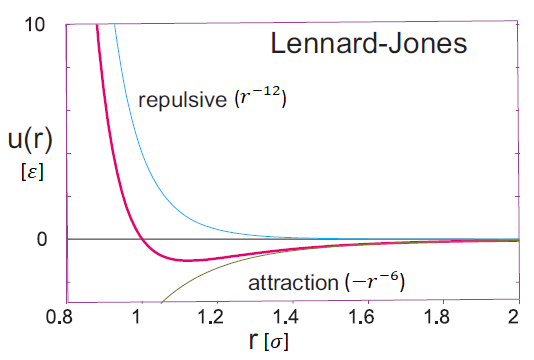
\includegraphics[width=0.6\linewidth]{media/LJ}
	\caption{A Lennard-Jones potenciál távolságfüggése $\sigma$ és $\varepsilon$ egységekben, a taszító és vonzó tag összegéből képezve. Ábra: \cite{Landau2012}.}
	\label{fig:lj}
\end{figure}



\subsection{A potenciál levágása}

A számítások egyszerűsítése érdekében a párpotenciálhoz minden esetben definiálnak egy levágási sugarat:

\begin{equation}
	u(r) = \begin{cases}
	\begin{array}{lr}
		4 (r^{-12} - r^{-6}), & \rm{ha} ~ r<r_{cut},\\
	    0,					  & \rm{ha} ~ r>r_{cut},
	\end{array}
	\end{cases}
\end{equation}
szemléltető példaként továbbra is a Lennard-Jones potenciálnál maradva.
Az egy részecskére ható erőhöz tehát csak a levágási sugáron belül lévő részecskék adnak járulékot. A potenciál így nem folytonos, az abból számolt erő (a potenciál deriváltja) pedig szinguláris a levágási sugár értékénél ($r= r_{cut}$). Az elviekben konzervatív potenciál így már nem az, vagyis az energiamegmaradás nem teljesül egzaktul. A gyakorlatban viszont a levágási sugarat kellőképpen nagynak választjuk ahhoz, hogy a környezetében az erő értéke elhanyagolható legyen az egyéb közelítési és numerikus hibákhoz képest, így az energiamegmaradás ne sérüljön lényegesen \cite{Landau2012}.


\subsection{Felületi jelenségek}

Molekuladinamikai szimulációk segítségével gyakran makroszkopikus rendszerek viselkedésére igyekszünk következtetni $10^{23}$ részecskeszámmal. Mivel ennek a részecskeszámnak csak a töredékét szimuláljuk egy véges térfogatban, lényeges a felületi jelenségek megfelelő kezelése\footnote{Minél kevesebb részecskét szimulálunk, annál nagyobb problémát jelenthetnek a mesterséges felületi jelenségek. Vegyünk például 1000 gázrészecskét egy $10\times 10 \times 10$ egység méretű kockában, azaz egy részecske pont egy térfogategységet töltsön be átlagosan. Így $10^3-8^3 = 488$ részecske a felület szomszédságában helyezkedik el, ez 49\%-a az összes részecskének. $10^6$ számú részecskénél ugyanilyen megfontolás mentén már csak a részecskék 6\%-a található a felület szomszédságában.}. Leggyakrabban periodikus határfeltételt alkalmazunk, az alábbiakban kizárólag ezt mutatom be. Ettől eltérő eset például a kapilláris csövekben modellezett dinamika, ahol kemény falat kell feltételezni, illetve biopolimerek szimulációjakor szükség lehet stohasztikus határfeltételre vagy határfeltétel nélküli (effektíve végtelen) szimulációs térfogatra \cite{lecture}. 

A periodikus határfeltétel esetében gyakorlatilag azt feltételezzük, hogy a szimulációban definiált térfogat/síkidom végtelenszer ismétlődik minden irányban (szemléltetésként lásd: \ref{fig:periodicboundary}. ábra). Ha egy integrálási lépés során egy részecske elhagyná a szimulációs térfogatot, az ellenkező oldalon "beléptetjük" az úgynevezett képét. Precízen arra az esetre, ha a szimulációs térfogat a $[0, ~L_x] \times [0, ~L_y] \times [0, ~L_z]$ téglatest, és a részecske $x$ koordinátája lép ki a lehetséges intervallumból:

\begin{equation}
	x \Rightarrow \begin{cases}
	\begin{array}{lr}
	x + L_x, & \rm{ha} ~x<0, \\
	x - L_x, & \rm{ha} ~x>0.
	\end{array}
	\end{cases}
	\label{eq:periodic}
\end{equation}
Valójában a periodikus határfeltétel ennél többet jelent: a valódi atomok mellett ugyanis azok képei is részt vehetnek párkölcsönhatásokban. Ez effektíve olyan, mintha végtelen számú részecskét szimulálnánk \cite{Landau2012}, miközben technikailag csak $N$ darab mozgásegyenletet integrálunk. Hogy mennyi képét kell számon tartani egy atomnak a kölcsönhatások számolásakor, az a párpotenciál levágási sugarától függ -- ez teszi a gyakorlatban végessé a párkölcsönhatások számát és a periodikusan kiterjesztett térfogatot. Ha a levágási sugár kisebb a szimulációs doboz egy adott oldalhosszának felénél ($r_{cut} < L_i/2$), elegendő egy képet nyilvántartani abban az irányban. Ilyenkor egy atom egy másik atomnak vagy a képével, vagy a valódi atommal hat kölcsön, attól függően, melyik van hozzá közelebb. Szemléltetésként lásd a \ref{fig:periodicboundary}. ábrán a kettős végű nyilakat. 


\begin{figure}
	\centering
	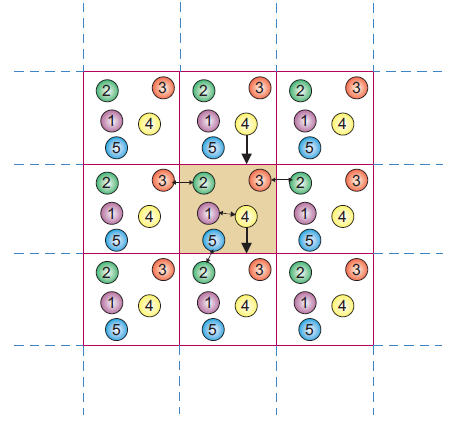
\includegraphics[width=0.5\linewidth]{media/periodic_boundary}
	\caption{A periodikus határfeltétel szemléltetése \cite{Landau2012}. Középen a valódi szimulációs térfogat, ami minden irányban ismétlődik. A 4-es számú részecskékhez tartozó függőleges nyilak a határon kilépő részecske ellenkező oldalon történő beléptetését jelzik (lásd: \ref{eq:periodic}. összefüggés), a kettős végű nyilak pedig azt mutatják, hogy a párkölcsönhatások számolásakor mikor vesszük az eredeti részecskéket, illetve valamelyiknek a képét ($r_{cut} < L_i/2$ esetben).}
	\label{fig:periodicboundary}
\end{figure}


\section{Integrálási algoritmusok}

A newtoni mozgásegyenletek integrálása közönséges differenciálegyenlet-rendszer lévén egzaktul megoldható numerikusan, sokféle integrálási sémával. Molekuladinamikai szimulációk során legelterjedtebben a Verlet- és sebesség-Verlet-algoritmusokat használjuk, az energiamegmaradás biztosítéka és a kiemelkedő stabilitás miatt.


\subsection{Verlet-algoritmus}

Egy részecske pozíciójának diszkrét léptetése $\tau$ időlépéssel, Taylor-sorfejtést alkalmazva:

\begin{equation}
	\mathbf{r}_i (t+\tau) = \mathbf{r}_i(t) + \mathbf{v}_i(t) \tau + \frac{1}{2} \mathbf{a}_i(t) \tau^2 + \frac{1}{6} \dddot{\mathbf{r}}_i (t) \tau^3 + \mathcal{O}(\tau^4).
	\label{eq:Taylor_pos}
\end{equation}
Ugyanígy, negatív időlépést ($-\tau$) véve:

\begin{equation}
	\mathbf{r}_i (t-\tau) = \mathbf{r}_i(t) - \mathbf{v}_i(t) \tau + \frac{1}{2} \mathbf{a}_i(t) \tau^2 - \frac{1}{6} \dddot{\mathbf{r}}_i (t) \tau^3 + \mathcal{O}(\tau^4).
	\label{eq:Taylor_neg}
\end{equation}
A fenti egyenleteket összeadva ((\ref{eq:Taylor_pos})~+~(\ref{eq:Taylor_neg})):

\begin{equation}
	\mathbf{r}_i (t+\tau) + \mathbf{r}_i (t-\tau) = 2 \mathbf{r}_i(t) + \mathbf{a}_i(t) \tau^2 + \mathcal{O}(\tau^4).
\end{equation}
Ezt átrendezve, a gyorsulást átírva a következő alternatív összefüggést kapjuk a pozíció léptetésére:

\begin{equation}
	\mathbf{r}_i (t+\tau) = 2 \mathbf{r}_i(t) - \mathbf{r}_i (t-\tau) + \frac{\mathbf{F}_i(\mathbf{r}_1 (t), \mathbf{r}_2 (t) \dots \mathbf{r}_N (t))}{m_i} \tau^2 + \mathcal{O}(\tau^4).
	\label{eq:Verlet_pos}
\end{equation}
Ez az egyenlet (\ref{eq:Verlet_pos}) adja a Verlet-algoritmus alapját \cite{lecture, Landau2012}. Használatával a sebesség kiszámolása nélkül, negyedrendű integrálási hibával adhatjuk meg a részecskék pályáját. Az erők számolása közvetlenül a részecskék pozícióiból történik, minden időlépésben. Az algoritmus integrálási sémáját \aref{fig:verlettimeline}. ábra szemlélteti. Mivel ebben a sémában az erőnek nincs explicit időfüggése -- nem integrálással számoljuk, hanem a részecskék pozícióiból, a konzervatív potenciál kiértékelésével --, a teljes energiamegmaradás teljesül, nem befolyásolja az integrálási hiba. Noha a sebesség kiszámolása nem szükséges a pálya követéséhez, molekuladinamikai szimulációkban általában szükség van a sebesség ismeretére (a teljes mozgási energia, illetve ebből a hőmérséklet számolásához, lásd később, a 4. fejezetben). Ez a középpontidifferencia-módszerrel számolható:

\begin{equation}
	\mathbf{v}_i(t) = \frac{\dd \mathbf{r}_i(t)}{\dd t} = \frac{\mathbf{r}_i(t+\tau) - \mathbf{r}_i(t-\tau)}{2 \tau} + \mathcal{O}(\tau^2).
	\label{eq:Verlet_vel}
\end{equation}
Megjegyzendő, hogy a Verlet-szimuláció kezdetén szükséges egy inicializáló integrálási lépés, mivel az algoritmus az új pozíciót két korábbi időlépésben felvett pozícióból számolja. Az inicializáció egyszerű Euler-lépéssel:

\begin{equation}
	\mathbf{r}_i(-\tau) = \mathbf{r}_i(0) - \mathbf{v}_i(0) \tau + \frac{1}{2} \frac{ \mathbf{F}_i(\mathbf{r}_1 (0), \mathbf{r}_2 (0) \dots \mathbf{r}_N (0))}{m_i} \tau^2 + \mathcal{O}(\tau^3).
	\label{eq:Verlet_init}
\end{equation}


\begin{figure}
	\centering
	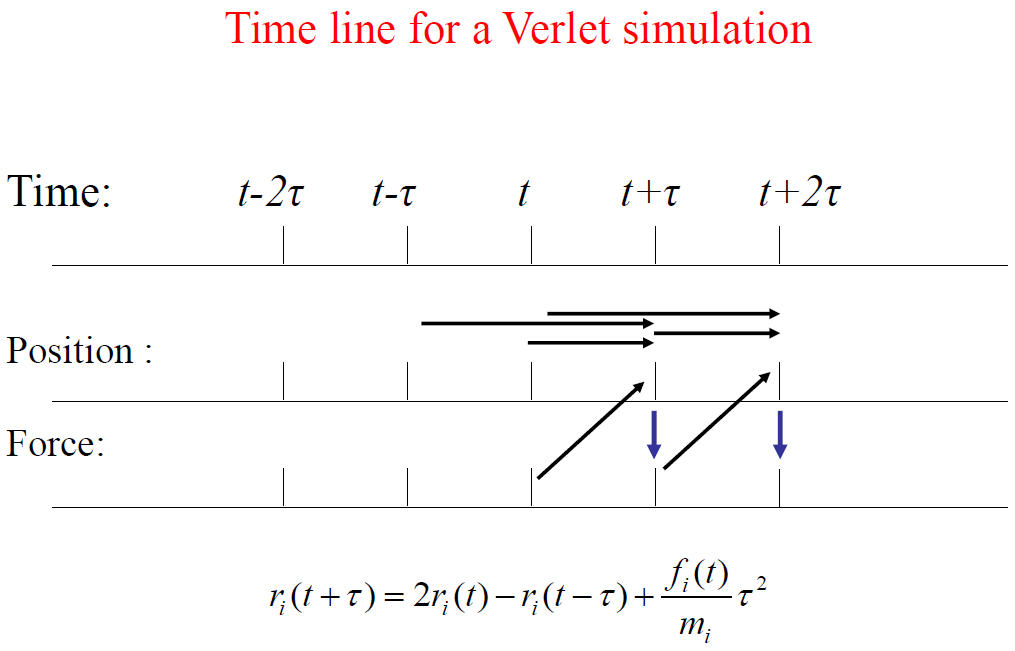
\includegraphics[width=0.5\linewidth]{media/Verlet_timeline}
	\caption{A pozíció léptetése és az erő számolása a Verlet-algoritmus során \cite{lecture}.}
	\label{fig:verlettimeline}
\end{figure}


\subsection{Sebesség-Verlet-algoritmus}

A Verlet-algoritmus másik verziója a sebesség-Verlet-algoritmus, ami explicit módon számolja a sebességet és használja fel az integráláshoz minden lépésben:

\begin{equation}
	\mathbf{r}_i (t+\tau) = \mathbf{r}_i(t) + \mathbf{v}_i(t) \tau + \frac{1}{2} \mathbf{a}_i(t) \tau^2 + \mathcal{O}(\tau^3),
	\label{eq:velVerlet_pos}
\end{equation}

\begin{equation}
	\mathbf{v}_i (t+\tau) = \mathbf{v}_i(t) + \overline{\mathbf{a}_i(t)} \tau + \mathcal{O}(\tau^2) =
	\label{eq:velVerlet_vel}
\end{equation}
\begin{equation*}
	~~~~~~~~~~~~~~~~~~~~~~~~~~~~~~ =\mathbf{v}_i(t) + \left[\frac{ \mathbf{a}_i(t+\tau) + \mathbf{a}_i(t)}{2}\right] \tau + \mathcal{O}(\tau^2).
\end{equation*}
Megjegyzendő, hogy az $\mathbf{a}_i(t)$ jelölésmód a gyorsulásra csak rövidítés: azt továbbra is az atomok pozíciójából, azaz implicit időfüggés alapján számoljuk, ahogy a (\ref{eq:Verlet_pos}) és (\ref{eq:Verlet_init}) számú összefüggésekben. A koordináták, a sebességek és az erő számolásának a fenti (\ref{eq:velVerlet_pos} és \ref{eq:velVerlet_vel}) összefüggések által meghatározott menetét \aref{fig:velverlettimeline}. ábra szemlélteti. A számolás pontosságát növeli, hogy a sebesség léptetésekor a gyorsulást az időlépés elején és végén lévő konfigurációból számolt érték átlagának vesszük, illetve, hogy az így számolt sebességet használjuk a koordináta következő léptetésekor. Ez ellensúlyozza azt a hátrányt, hogy a sebesség-Verlet-algoritmus hibája a koordináta léptetésére alacsonyabb rendű a Verlet-algoritmushoz képest (harmadrendű vs negyedrendű), és végeredményben a két algoritmus hasonló pontosságot eredményez \cite{Landau2012}. Ahogy az látható, a számolás során a koordinátákat mindig előbb kell léptetnünk, mint a sebességet. A koordináták léptetéskor fontos szerepe van a periodikus határfeltételnek, hiszen módosítja az atomokra ható erőt, így a sebesség közvetlen utána következő léptetését. A határokon történő ellenőrzést tehát a pozíció léptetése után, a sebesség léptetése előtt kell elvégezni.


\begin{figure}
	\centering
	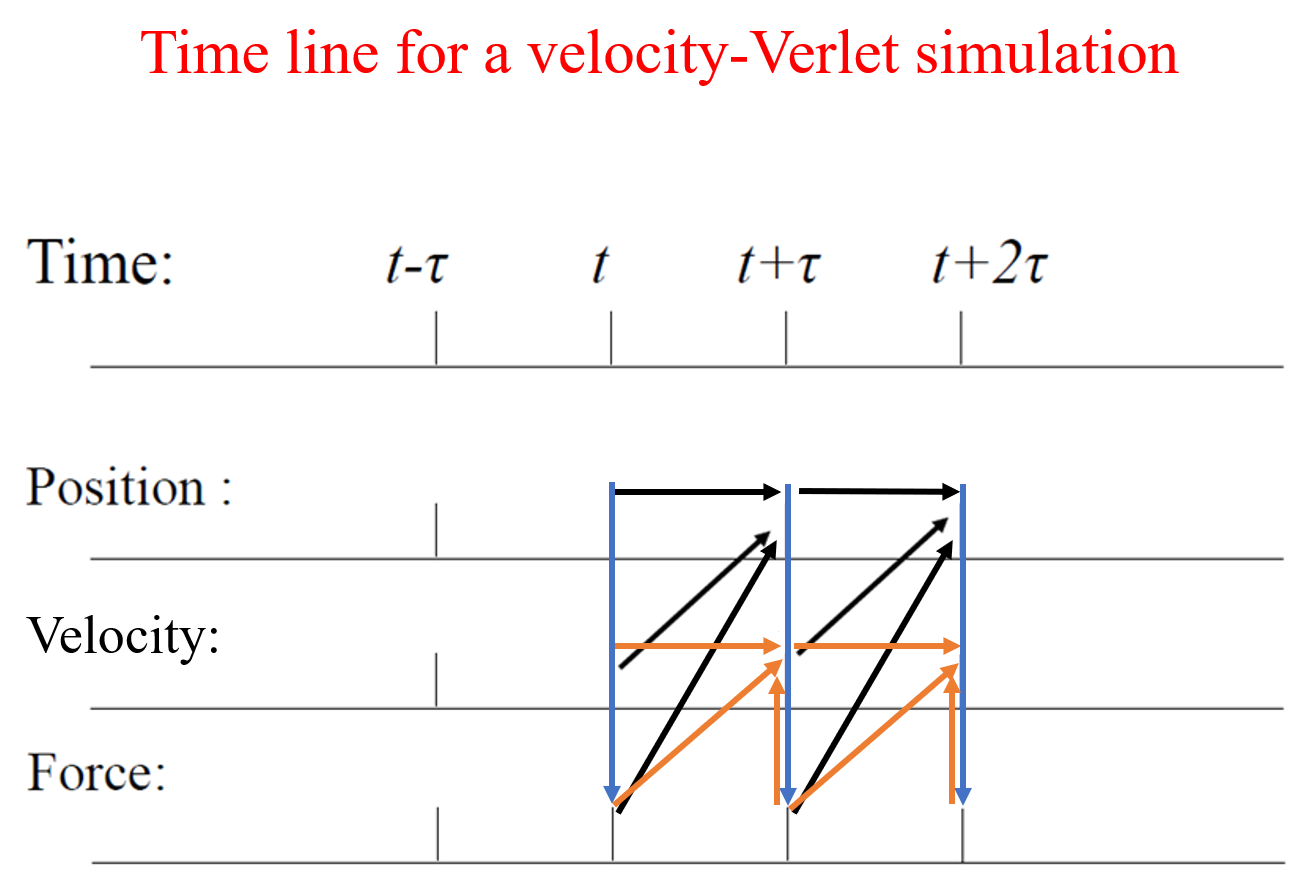
\includegraphics[width=0.5\linewidth]{media/velVerlet_timeline}
	\caption{A pozíció, a sebesség és az erő számolásának menete a sebesség-Verlet-algoritmus során.}
	\label{fig:velverlettimeline}
\end{figure}



\section{Termodinamikai mennyiségek meghatározása}

Egy rendszer részecskéinek trajektóriáit -- mikroszkopikus viselkedését -- követő molekuladinamikai szimuláció eredményeit a statisztikus fizika törvényei alapján  hozhatjuk kapcsolatba a makroszkopikus termodinamikai paraméterekkel. Ehhez elegendően nagy számú részecskére van szükség. A sokrészecske-rendszer teljes transzlációs kinetikus energiája egy adott konfigurációban (időlépésben) a szimulációból a következő egyszerű összegzés szerint kapható:

\begin{equation}
	KE = \sum_{i=1}^{N} \frac{1}{2} m_i v_i^2.
	\label{eq:Ekin}
\end{equation}
Az ekvipartíció tétele szerint a hőmérséklet és a transzlációs kinetikus energia kapcsolata:

\begin{equation}
	\braket{KE} = N \frac{d}{2} k_B T,
	\label{eq:equipart}
\end{equation}
ahol $d$ a térbeli dimenzió (a gyakorlatban 2 vagy 3), a $\braket{KE}$ jelölés pedig a mozgási energia időátlagát jelenti. Az időátlag azért lényeges, mert a kinetikus és potenciális energia egy bizonyos érték körül fluktuál az egyensúlyi szimulációban, azoknak csak az összege állandó, így egy időpillanatra vonatkozó adat nem releváns az egyensúlyi hőmérsékletre nézve. A hőmérséklet a fenti egyenlet (\ref{eq:equipart}) alapján:

\begin{equation}
	T = \frac{2 \braket{KE}}{k_B d N}.
	\label{eq:temperature}
\end{equation}
A nyomás a Viriál-tétel felhasználásával számolható \cite{Landau2012, LAMMPS_compute_pressure}:

\begin{equation}
	p V = N k_B T + \frac{w}{d},
	\label{eq:Virial_theorem}
\end{equation}
ahol 

\begin{equation}
	w = \Braket{\sum_{i<j}^{N} \mathbf{r}_{ij} \cdot \mathbf{f}_{ij}}
	\label{eq:Virial}
\end{equation}
a viriál, az összes párkölcsönhatásból származó erő nyomatéka időátlagban. Az összegzés során minden részecskepárt csak egyszer számolunk, és a 2.2 fejezetben elmondottak szerint a részecskék képei is adhatnak járulékot az eredeti részecskék helyett/mellett. Az időátlag ismét a fluktuációk kiküszöbölése érdekében szükséges. A nyomás tehát, a (\ref{eq:temperature}) és (\ref{eq:Virial_theorem}) számú összefüggéseket felhasználva, a szimulációból közvetlenül számolható mennyiségekkel kifejezve:

\begin{equation}
	p = \frac{1}{V d} (2 \braket{KE} + w).
	\label{eq:pressure}
\end{equation}


\section{Relaxáció}

Molekuladinamikai szimulációval egyaránt modellezhető egyensúlyi és nemegyensúlyi folyamatok dinamikája, és a célnak megfelelően különféle -- esetenként bonyolult és egyedi -- kezdőfeltételeket lehet implementálni. A legegyszerűbb típusú szimuláció, amikor valamilyen random vagy mesterségesen rendezett kezdeti állapotból egyensúlyi állapotba relaxáltatjuk a rendszert. Ilyenkor alapesetben mikrokanonikus sokaságnak tekinthető a rendszer, hiszen a részecskék száma, a szimulációs térfogat és a teljes energia állandó \cite{Landau2012}; a szimuláció során folyamatos átmenet van a kinetikus és potenciális energia között, és a kettő aránya végül egy állandó érték körül fluktuál bizonyos hibahatáron belül. 

Hogy csak egy egyszerű példát vegyünk: gáz halmazállapotú rendszer szimulációjakor például lehet egy bizonyos hőmérsékletnek megfelelő Maxwell-Boltzmann eloszlásból random kezdősebességet generálni a gázrészecskéknek, majd a newtoni dinamika szerint mozgatva őket megvárni az egyensúlyi állapot kialakulását az adott hőmérsékleten\footnote{Amikor egy bizonyos hőmérsékletnek megfelelő Maxwell-Boltzmann-eloszlásból generálunk sebességet a részecskéknek, az korántsem egyensúlyi helyzet, hiszen a mozgás ilyenkor teljesen korrelálatlan.}. A hőmérséklet rögzítésére egyszerű megoldás a sebességskálázás: a hőmérsékletdrift elkerülése érdekében az atomok mozgási energiáját a szimuláció elején bizonyos időlépésenként úgy növeljük vagy csökkentjük egységesen egy szorzófaktorral, hogy a pillanatnyi hőmérséklet megfeleljen a kívánt egyensúlyi hőmérsékletnek. Azaz:

\begin{equation}
	\mathbf{v}_i'(t) = s \cdot \mathbf{v}_i(t),
\end{equation}
ahol

\begin{equation}
	s = \sqrt{\frac{T_{eq}}{T(t)}}
\end{equation}
a skálafaktor, $T_{eq}$ a kívánt egyensúlyi, $T(t)$ a pillanatnyi hőmérséklet. A skálafaktor hőmérsékletek arányától való gyökös függéséhez lásd a (\ref{eq:Ekin}) és (\ref{eq:temperature}) számú összefüggéseket. Az egyensúlyi állapotba történő relaxáció után már nincs szükség a sebességskálázásra, a kinetikus és potenciális energia, és így a hőmérséklet is az egyensúlyi értékük körül fluktuál. Az állandó fluktuáció miatt termodinamikai mennyiségek számolásához minél hosszabban kell futtatni a számolást, hogy az így képzett időátlagok (lásd: (\ref{eq:temperature}), (\ref{eq:Virial})) hibája minél kisebb legyen ($\rm{Err} \propto \frac{1}{\sqrt{N}}$ szerint).

A gyakorlatban a fent ismertetett sebességskálázásnál bonyolultabb módszerekkel biztosítjuk a rendszer megfelelő egyensúlyi állapotba való relaxációját: a célnak megfelelően úgynevezett termosztátokat/barosztátokat lehet alkalmazni az atomok egy csoportjára vagy a rendszer egészére, amelyek megadják, hogy a hőmérséklet/nyomás milyen értékhez konvergáljon, illetve, hogy az integrálás során ez milyen numerikus módszerrel legyen biztosítva (pl. Langevin termosztát, 300 K hőmérséklet \cite{LAMMPS_fix_langevin}). Ennek részletei túlmutatnak a tétel mélységein, az érdeklődők számára a bevett és széles körben alkalmazható nyílt forrású LAMMPS szoftver dokumentációját ajánlom kiindulópontnak: \cite{LAMMPS_howto_thermostat, LAMMPS_howto_barostat}.


%\begin{figure}[H]
%    \begin{center}
%    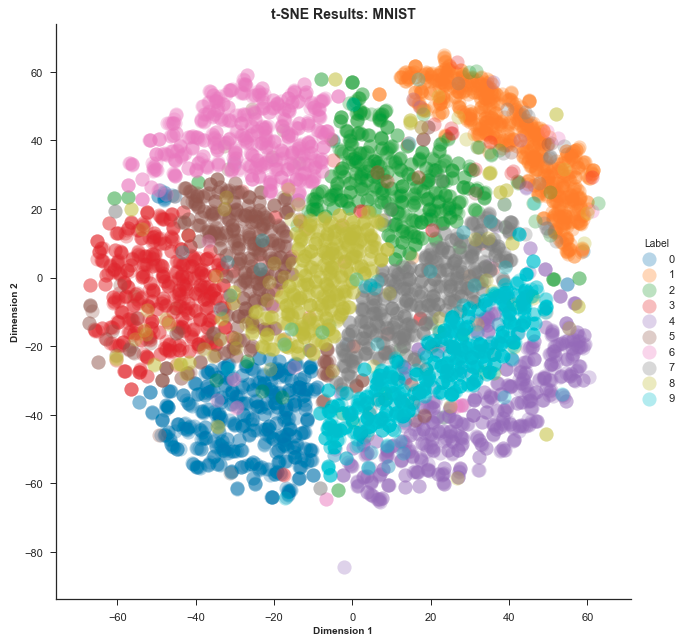
\includegraphics[width=0.5\textwidth]{media/tsneplot.png}
%    \caption{t-SNE plot for MNIST dataset \cite{tsne-article}} 
%    \label{fig:tsneplot}
%    \end{center}
%\end{figure}


\bibliographystyle{plain}
%\bibliographystyle{unsrt}
%\bibliographystyle{ieeetr}
\bibliography{references}

\end{document}
